In the course of all the described experiments, the performance of both the simple and the complex Texter were steadily improved. What was missing was the hoped-for increase in performance of the attentive Texter compared to the simple version. Instead, the simple Texter actually performs better on many text sets. In order to get to the bottom of the cause, the attention mechanism should be investigated to find out whether the basic assumption that the class embeddings react to sentences in which class-typical keywords appear can be verified. In particular, it was examined (1) whether the trained class embeddings match keywords that are typical for the respective class, (2) whether the attention block favors sentences that would yield clear classification results on their own and (3) how the attention value related to a sentence results from the sentence's individual words.

Regarding the first question, the assumption was that the class embeddings converge against keywords that are particularly meaningful for a class during training. To confirm this conjecture, the class embeddings $class_c$, of a trained texter were scalar multiplied with all word embeddings $word_w$ of the vocabulary, the resulting scalar products $\langle class_c, word_w \rangle$ were sorted, and the values with the largest absolute values $|\langle class_c, word_w \rangle|$ were examined for plausibility. Thereby, the indices $1 <= c <= |C|$ and $1 <= w <= |V|$ specify one of the classes from the class set $C$ and a word from the vocabulary $V$, respectively. It was expected that among these top candidates mainly words would be found that clearly speak for or against the corresponding class. Table shows the top words the attentive Texter reacts to after being trained on the CDE split with cde-irt-5-clean texts.

\begin{table}[h]
    \makebox[\textwidth][c]{
        \begin{tabular}{ l l }
    \toprule

    \multicolumn{1}{l}{\textbf{Class}} &
    \multicolumn{1}{l}{\textbf{Top matching words}} \\

    \midrule

    $(x, from, USA)$ & nhs, mid-engined, ruislip, filipina   \\
    $(x, is, writer)$                               & recepter, 1/4, makovsky, pairwise     \\
    $(x, speaks, English)$    & republish, in-demand, brahmos, steyr \\

    \bottomrule
\end{tabular}

    }
    \caption{Top words matching the static, attentive Texter's classes}
    \label{tab:5_experiments/4_texter/2_static/9_attention/top_words}
\end{table}

Contrary to the assumption, the top words do not show a clear relation to the respective classes. With a few exceptions such as "Maryland" and "BBC" which appear further down in the suggestions for (from, USA) or (speaks, English), the words appear rather random. Given the rather infrequent occurrence of top words, overfitting seemed the most obvious explanation. However, the top words change with repeated training runs, so it seemed more likely that the word embeddings simply happened to be close to the learned class embeddings. As long as this only affects a small proportion of top words and the class embeddings are mostly close to relevant words, this should have little impact on the generalizability of the model. Whether this relation exists to more frequent keywords was investigated in the third experiment.

Before that, the second question was clarified whether the attention mechanism weights the sentences most heavily that are also the most meaningful on their own. For this purpose, the attentive Texter was extended by a method that bypasses the attention mechanism during inference. The trained model is still passed multiple sentences per entity when called, but instead of these being calculated entity embeddings in the attention block, the sentence embeddings are pushed directly through the classification block. That function, denoted as $\psi$ in the following, finally returns the non-aggregated class logits for each individual sentence. However, since the linear layers of the complex model were actually trained on the entity embeddings, this experiment only works with a texter in whose attention block the softmax function is used. This is because the Sigmoid version, unlike the Softmax version, does not have the property that the individual set embeddings have the same order of magnitude as the entity embeddings. Therefore, the results of the attentive model trained with Softmax on the cde-irt-5-clean texts are shown below. However, since the performance of the Softmax version is almost as high as that of the Sigmoid version, the results should be representative. Table~\ref{tab:5_experiments/4_texter/2_static/9_attention/kari_soft} presents exemplary values for the entity Kari Hotakainen, a Finnish writer. In addition to the five rather short sentences about Kari as well as the model predictions and the ground truth concerning the four most frequent classes in the CDE split, for each class-sentence combination it is stated to which proportion the sentence embedding normally enters into the entity embedding and which result the function $\psi$ yields when the attention mechanism is bypassed. Considering only the selected classes, the positive predictions for logits above the zero threshold in the example result in a precision of 33\%, a recall of 100\%, and thus an overall F1 score of 33\% and thereby close to the cde-irt-5-clean text set's average value of 37.6\%. However, it must be mentioned that the observable effectiveness of the attention mechanism is rather above average. The example was chosen mainly because of the short sentences.

\begin{table}[h]
    \centering
    \begin{tabular}{|l|l|r|r|r|r|}
\hline
\multicolumn{1}{|c|}{\multirow{2}{*}{\textbf{Sentence}}} &
   &
  \multicolumn{4}{c|}{\textbf{Class}} \\ \cline{2-6} 
\multicolumn{1}{|c|}{} &
   &
  \multicolumn{1}{c|}{\textbf{\begin{tabular}[c]{@{}c@{}}from\\ USA\end{tabular}}} &
  \multicolumn{1}{c|}{\textbf{\begin{tabular}[c]{@{}c@{}}is\\ writer\end{tabular}}} &
  \multicolumn{1}{c|}{\textbf{\begin{tabular}[c]{@{}c@{}}speaks\\ English\end{tabular}}} &
  \multicolumn{1}{c|}{\textbf{\begin{tabular}[c]{@{}c@{}}is\\ actor\end{tabular}}} \\ \cline{2-6} 
 &
  $\phi_c(S)$ &
  -1.26 &
  1.98 &
  0.22 &
  0.55 \\ \cline{2-6} 
 &
  GT &
  \multicolumn{1}{c|}{0} &
  \multicolumn{1}{c|}{1} &
  \multicolumn{1}{c|}{0} &
  \multicolumn{1}{c|}{0} \\ \hline
\begin{tabular}[c]{@{}l@{}}the film was written by\\ kari \_ and juha \_\end{tabular} &
  \multirow{5}{*}{\begin{tabular}[c]{@{}l@{}} \\ \\ \\ \\ $\sigma(\langle e_c, e_s \rangle)$ \\ $\psi_c(s)$\end{tabular}} &
  \begin{tabular}[c]{@{}r@{}} 0.16 \\ -0.16 \end{tabular} &
  \begin{tabular}[c]{@{}r@{}} 0.11 \\  2.01 \end{tabular} &
  \begin{tabular}[c]{@{}r@{}} 0.12 \\  0.88 \end{tabular} &
  \begin{tabular}[c]{@{}r@{}} 0.13 \\  0.11 \end{tabular} \\ \cline{1-1} \cline{3-6} 
\begin{tabular}[c]{@{}l@{}}it is based on kari \_ semi-\\ autobiographical novel \_\end{tabular} &
   &
  \begin{tabular}[c]{@{}r@{}} 0.22 \\ -1.06 \end{tabular} &
  \begin{tabular}[c]{@{}r@{}} \textbf{0.27} \\  \textbf{2.69} \end{tabular} &
  \begin{tabular}[c]{@{}r@{}} 0.21 \\  0.57 \end{tabular} &
  \begin{tabular}[c]{@{}r@{}} 0.22 \\ -0.06 \end{tabular} \\ \cline{1-1} \cline{3-6} 
\begin{tabular}[c]{@{}l@{}}the film is inspired by kari \\ \_ novel of the same name.\end{tabular} &
   &
  \begin{tabular}[c]{@{}r@{}} 0.12 \\  0.16 \end{tabular} &
  \begin{tabular}[c]{@{}r@{}} 0.26 \\  2.40 \end{tabular} &
  \begin{tabular}[c]{@{}r@{}} 0.17 \\  \textbf{1.24} \end{tabular} &
  \begin{tabular}[c]{@{}r@{}} 0.11 \\  0.02 \end{tabular} \\ \cline{1-1} \cline{3-6} 
\begin{tabular}[c]{@{}l@{}}the unknown \_ \_ () is an\\ authorised biography on \\ finnish racing driver \_ \_ \\ by kari \_\end{tabular} &
   &
  \begin{tabular}[c]{@{}r@{}} \textbf{0.32} \\ \textbf{-2.87} \end{tabular} &
  \begin{tabular}[c]{@{}r@{}} 0.23 \\  1.04 \end{tabular} &
  \begin{tabular}[c]{@{}r@{}} \textbf{0.29} \\ -0.64 \end{tabular} &
  \begin{tabular}[c]{@{}r@{}} 0.26 \\  1.01 \end{tabular} \\ \cline{1-1} \cline{3-6} 
\begin{tabular}[c]{@{}l@{}}\_ is a 2002 novel by \\ finnish author kari \_\end{tabular} &
   &
  \begin{tabular}[c]{@{}r@{}} 0.18 \\ -0.57 \end{tabular} &
  \begin{tabular}[c]{@{}r@{}} 0.13 \\  1.24 \end{tabular} &
  \begin{tabular}[c]{@{}r@{}} 0.22 \\ -0.07 \end{tabular} &
  \begin{tabular}[c]{@{}r@{}} \textbf{0.28} \\  \textbf{1.03} \end{tabular} \\ \hline
\end{tabular}

    \caption{Result when predicting facts for the example entity Kari Hotakainen using the static, attentive Texter with Softmax - $\phi_c(S)$ and GT give the model's logits and ground truth for the whole entity while $\sigma(\langle e_c, e_s \rangle)$ and $\psi_c(s)$ are the class-sentence attentions and model logits when the attention mechanism is skipped, respectively}
    \label{tab:5_experiments/4_texter/2_static/9_attention/kari_soft}
\end{table}

For the exmample entity, the attentive Texter does indeed prefer those sentences that would give a clear result on their own in case of three of the four classes. In the fourth case, the model heavily incorporates a sentence that has a rather uncertain outcome. Despite that the respective prediction would have been correct on its own, the model should not have focused on it. Looking at other sentences that have been heavily weighted, further misjudgments become apparent, such as the cases where the texter relied on the fifth and second sentences to predict the classes (speaks, English) and (is, actor), respectively, which both lead to unreliable decisions on their own. Overall, however, it is noticeable that meaningful sentences are more strongly included in the entity embeddings.

However, the effective focus on sentences with a clear prediction alone is of no use if the unambiguous decision made on the basis of the individual sentences is wrong. For example, in Table~\ref{tab:5_experiments/4_texter/2_static/9_attention/kari_soft}, the first three sentences incorrectly indicate that Kari Hotakainen speaks English. Also, he is predicted to be an actor which is not the case which is probably due to the (is, actor) class's general high posterior probability as the dataset contains many actors. Otherwise, the sentences lead to largely correct classifications and was less certain about its two false positives than about its two correct predictions.

What is still missing, however, is a clear prioritization of the sentences. For example, as a human being, one would give the last sentence a much higher weighting when it comes to the negation of the class (from, USA) due to the fragment "by finnish author kari hotakainen". But, using static word embeddings, the model cannot recognize at this point that the word "finnish" is much more relevant than in the preceding sentence in which the same word does not refer to the entity itself. When the experiment is repeated, it is also noticeable that the class logits for the entire entity fluctuate only slightly, but change noticeably between individual sentences, which also changes the prioritization of the sentences.

This uncertainty about the order of the sentences also exists in the final model that uses the sigmoid function, although to a lesser extent. Table~\ref{tab:5_experiments/4_texter/2_static/9_attention/kari} shows, analogous to Table~\ref{tab:5_experiments/4_texter/2_static/9_attention/kari_soft}, the attention values after the sigmoid function has been applied instead of the softmax, which is why the probabilities no longer sum up to 100\% columnwise. Furthermore, Table~\ref{tab:5_experiments/4_texter/2_static/9_attention/kari_soft} misses the results of the $\psi$ function which cannot be calculated here as explained before. The shown figures imply that the sigmoid version achieves a higher overall precision due to the correct prediction of (is, actor) and that the inclusion of uncertain sentences is generally lower, but even here the order between the relevant sentences varies among training runs.

\begin{table}[h]
    \centering
    \begin{tabular}{| l | l | r r r r |}
\hline
\multicolumn{1}{|c|}{\multirow{2}{*}{\textbf{Sentence}}} &
   &
  \multicolumn{4}{c|}{\textbf{Class}} \\ \cline{3-6}
\multicolumn{1}{|c|}{} &
   &
  \multicolumn{1}{c}{\textbf{\begin{tabular}[c]{@{}c@{}}from\\ USA\end{tabular}}} &
  \multicolumn{1}{c}{\textbf{\begin{tabular}[c]{@{}c@{}}is\\ writer\end{tabular}}} &
  \multicolumn{1}{c}{\textbf{\begin{tabular}[c]{@{}c@{}}speaks\\ English\end{tabular}}} &
  \multicolumn{1}{c|}{\textbf{\begin{tabular}[c]{@{}c@{}}is\\ actor\end{tabular}}} \\ \cline{2-6}
 &
  \multicolumn{1}{c|}{$\phi_c(S)$} &
  -1.43 &
  2.19 &
  0.85 &
  -0.14 \\
 &
  \multicolumn{1}{c|}{GT} &
  \multicolumn{1}{r}{0} &
  \multicolumn{1}{r}{1} &
  \multicolumn{1}{r}{0} &
  \multicolumn{1}{c|}{0} \\ \hline
\begin{tabular}[c]{@{}l@{}}the film was written by\\ kari \_ and juha \_\end{tabular} &
  \multirow{5}{*}{\begin{tabular}[c]{@{}l@{}} \\ \\ \\ \\ $\sigma(\langle e_c, e_s \rangle)$ \end{tabular}} &
  0.47 &
  \textbf{0.74} &
  0.27 &
  0.36 \\ \cline{1-1} \cline{3-6} 
\begin{tabular}[c]{@{}l@{}}it is based on kari \_ semi-\\ autobiographical novel \_\end{tabular} &
   &
  0.40 &
  0.54 &
  0.23 &
  0.23 \\ \cline{1-1} \cline{3-6} 
\begin{tabular}[c]{@{}l@{}}the film is inspired by kari \\ \_ novel of the same name.\end{tabular} &
   &
  0.36 &
  0.45 &
  \textbf{0.13} &
  \textbf{0.21} \\ \cline{1-1} \cline{3-6} 
\begin{tabular}[c]{@{}l@{}}the unknown \_ \_ () is an\\ authorised biography on \\ finnish racing driver \_ \_ \\ by kari \_\end{tabular} &
   &
  0.31 &
  0.62 &
  0.20 &
  0.30 \\ \cline{1-1} \cline{3-6} 
\begin{tabular}[c]{@{}l@{}}\_ is a 2002 novel by \\ finnish author kari \_\end{tabular} &
   &
  \textbf{0.27} &
  0.57 &
  0.27 &
  0.38 \\ \hline
\end{tabular}

    \caption{Result when predicting facts for the example entity Kari Hotakainen using the static, attentive Texter with sigmoid - $\phi_c(S)$ and GT give the model's logits and ground truth for the whole entity while $\sigma(\langle e_c, e_s \rangle)$ denotes the class-sentence attentions}
    \label{tab:5_experiments/4_texter/2_static/9_attention/kari}
\end{table}

Another interesting insight is provided by the third experiment on the attention mechanism, which investigates how attention values derive from word embeddings. Prerequisite for the experiment is the usage of mean pooling, i.e. the calculation of the sentence embeddings as the mean of the respective word embeddings. In this case the scalar product of a class embedding $class_c$ and a sentence embedding $sent_s$ can be broken down to the mean of the scalar products between the class embedding and the sentence's word embeddings $word_w$ where $1 <= w <= N$ is the words position within the sentence:

\[
    \langle class_c, sent_s \rangle
    = \langle class_c, \frac{1}{N} \sum_{w=1}^N word_w \rangle
    = \frac{1}{N} \sum_{w=1}^N \langle class_c, word_w \rangle
\]

Leveraging this relationship, Figure~\ref{fig:5_experiments/4_texter/2_static/9_attention/kari_softmax} illustrates which words influence the overall scalar products between the class and sentence embeddings of the example entity Kari Hotakainen the most. Words that have a similar or opposite embedding to the class embedding are highlighted in yellow and purple, respectively. The expectation was that class-specific keywords would play a large role. During the experiment, it was noticed by coincidence that the result for Softmax- and Sigmoid-based attention mechanisms differ significantly. Therefore, each sentence is shown twice per class - once for Softmax and once for Sigmoid.

\begin{figure}
    \centering
    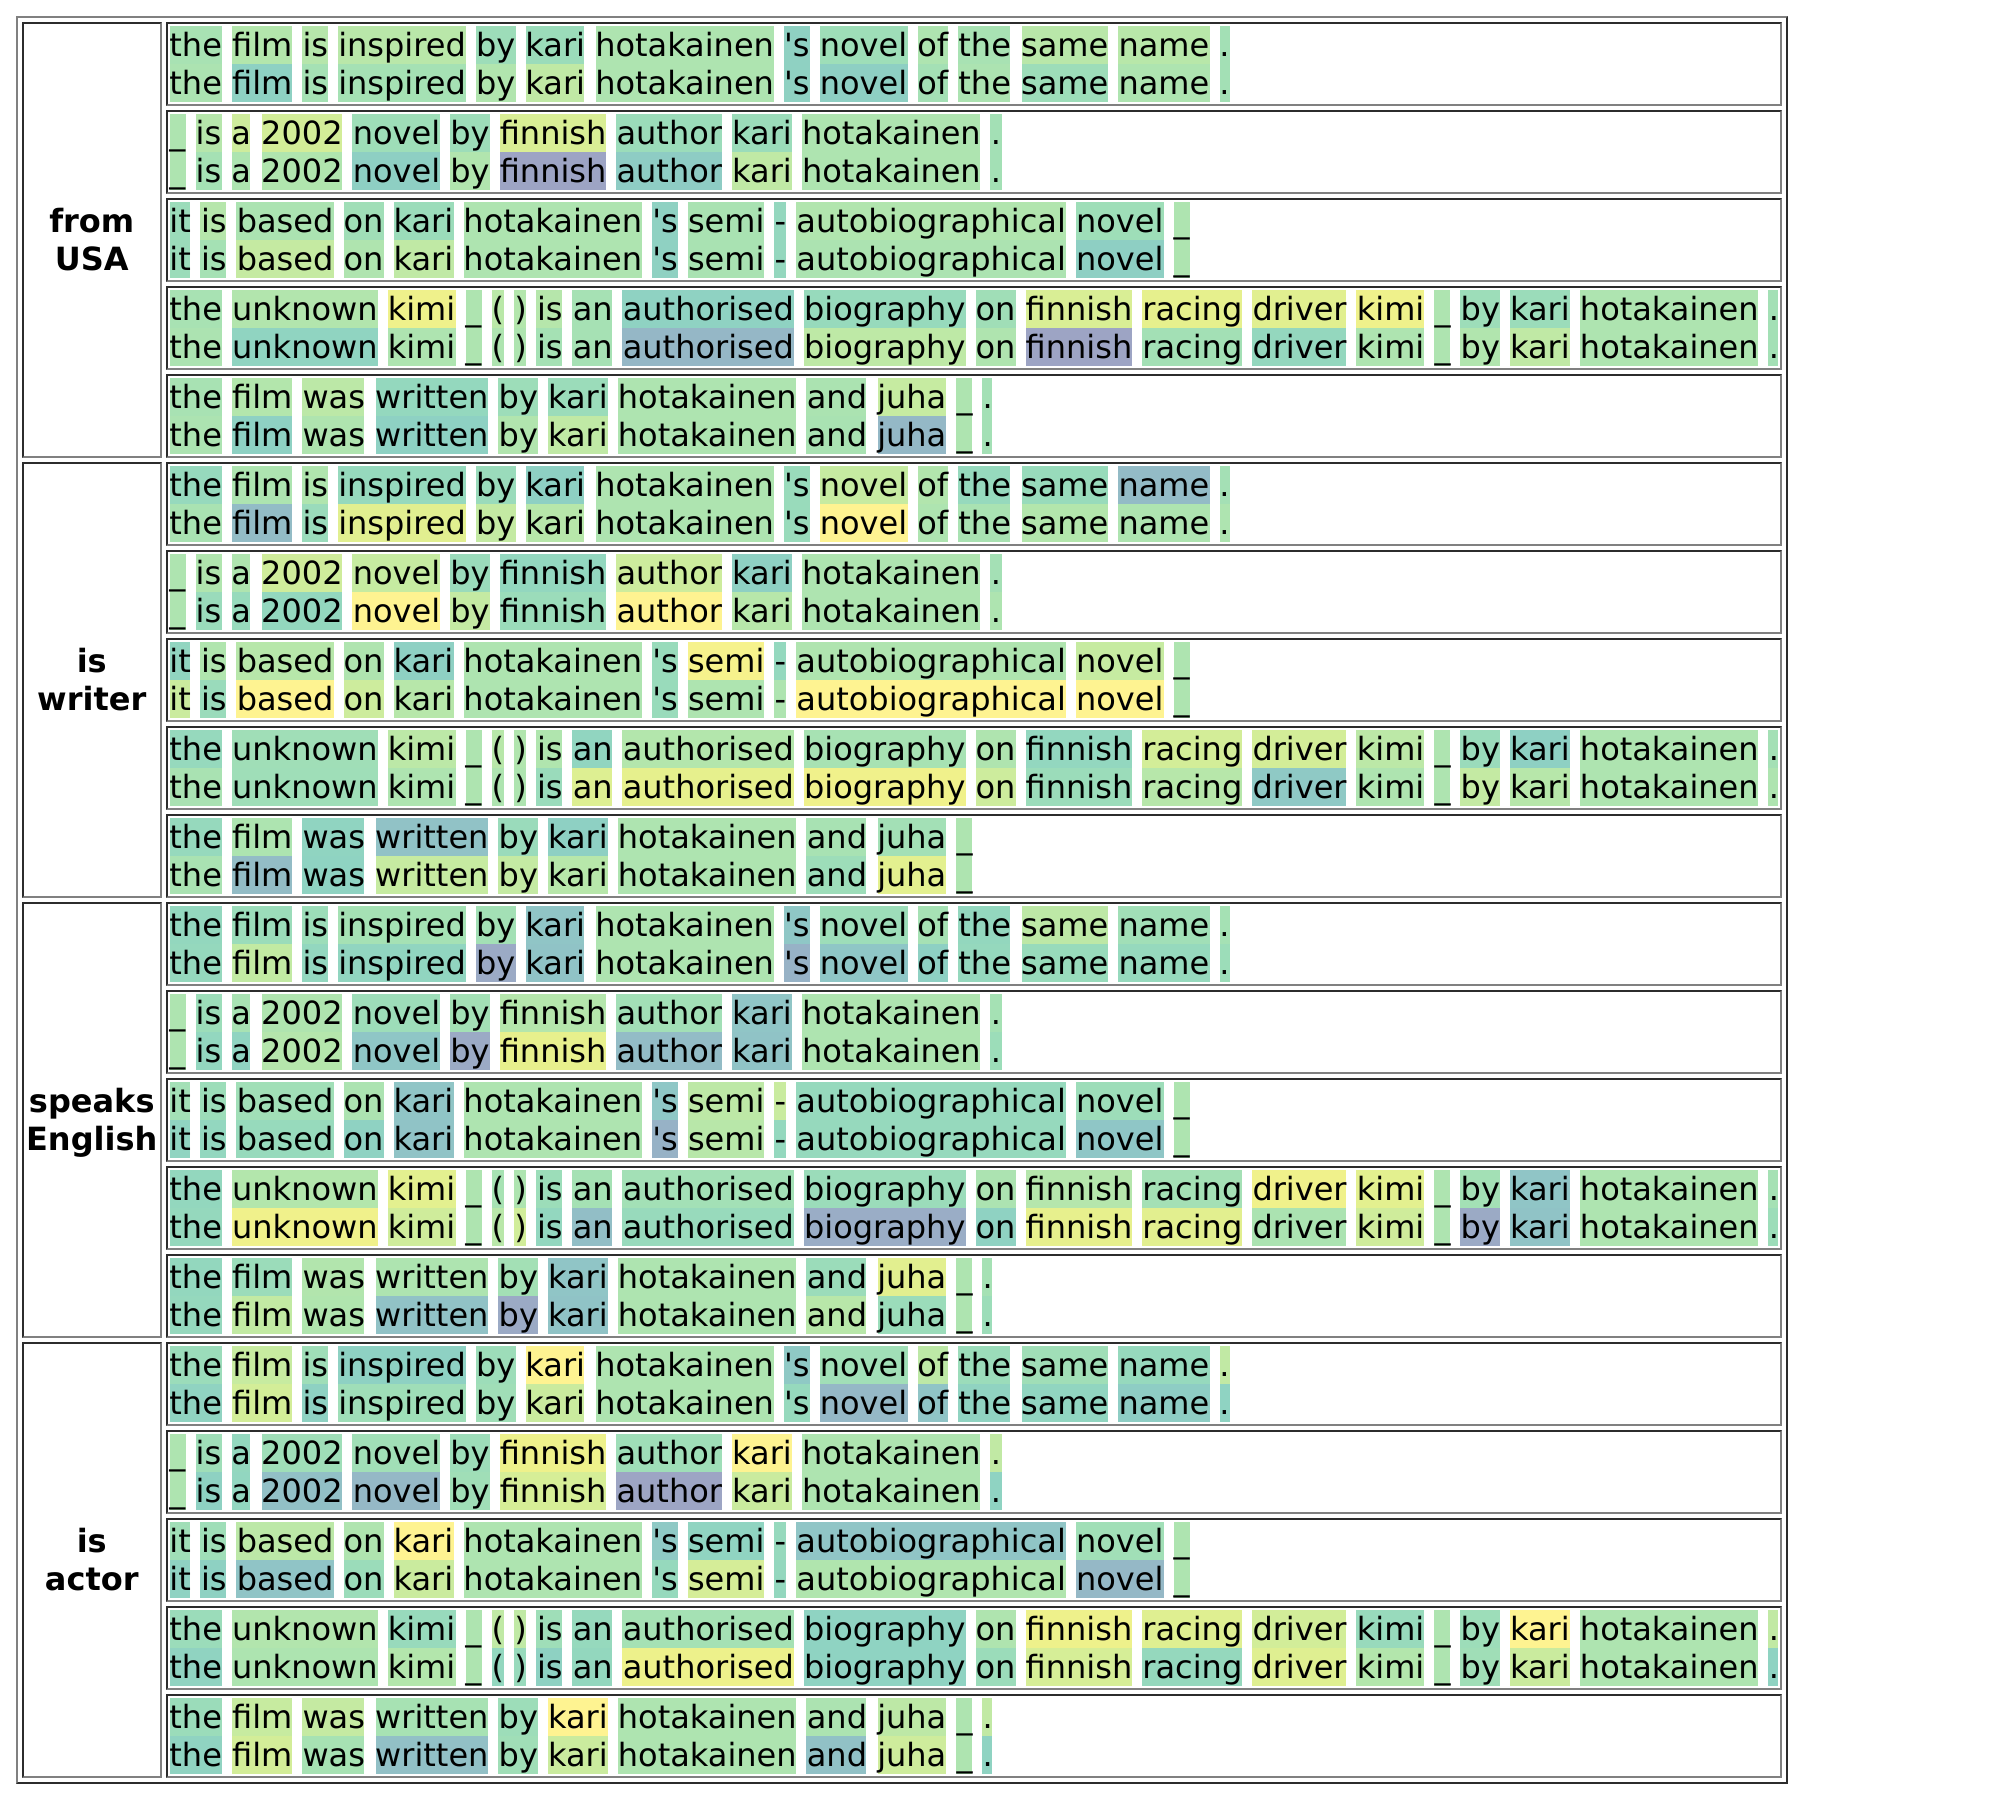
\includegraphics[width=\textwidth]{5_experiments/4_texter/2_static/9_attention/kari_softmax}
    \caption{Illustration of how the attention values for the example entity Kari Hotakainen can be traced back to class-related keywords that influence the overall sentence embeddings - low/high class-word attentions are highlighted in purple/yellow}
    \label{fig:5_experiments/4_texter/2_static/9_attention/kari_softmax}
\end{figure}

Although the use of the softmax or the sigmoid function in the attention block leads to very similar F1 scores the training of the word embeddings seems to differ significantly in both cases. When using sigmoid, the learned class embeddings attend on class-relevant keywords as expected whereas this is not the case with softmax. For example, the sigmoid version learns that the words "novel," "author," and "biography" are closely related to class (is, author) and that Finns tend to be likely to speak English. Conversely, "Finnish" and the name "Juha" militate against an origin from the US, and, apparently, authors are rarely actors at the same time. On the other hand, the softmax version attends to the names "Kimi" and "Kari" whose causal relationsships to (from, USA) and (is, actor) is less obvious.

In summary, the assumptions regarding the attention mechanism are only partially supported empirically and no reliable prioritization between an entity's sentences is established, which is probably the reason for the missing performance improvement of the attentive Texter compared to the attention-less version. One possible reason has already been mentioned: With static word embeddings it is not possible for the model to detect whether a potentially class-relevant keyword refers to the entity or not. This becomes even more obvious with a long sentence like the following of which there are many in the IRT text sentences:

\begin{displayquote}
    The Chilean writer Ricardo Cuadros said that McOndo irreverence for Latin American literary tradition, its thematic–stylistic concentration upon the pop culture of the United States, and the literatures’ apolitical tone, are dismissive of the literary ideas, writing style, and narrative techniques of the generation of Latin American writers (García Márquez, Vargas Llosa, Carpentier, Fuentes, et al.) who lived under, opposed, and (occasionally) were repressed by dictators.
\end{displayquote}

The sentece is associated with a Latin American writer who was classified as an American due to the keywords "United", "States" and the twice occurring "American" whose relation to "Latin" cannot be captured by static word embeddings. When trying to identify the entity in question, a second problem reveals itself in long sentences: Even as a human, it is not recognizable that, with all the named entities, the text is about the Peruvian writer Mario Vargas Llosa and not the Chilean Ricardo Cuadros. To address these problems, the next step is to use transformers that can recognize relationships between words and include special markers in the text sets that have not been used so far.
